\par Data used for this analysis was collected by the ATLAS detector during Run I 
of the LHC, with parameters and conditions set as discussed 
in Chapter~\ref{expSetup}. Only data from runs during which proton beams were stable were considered. 
The total integrated luminosity amounted to 20.2~\ifb. All of the data was collected 
during 2012. The total uncertainty on the luminosity value is 2.1\%. The impact of this uncertainty on  
final results in this search are discussed in Section~\ref{sec:exclHUnc}.  

\par The expected signal (Figure~\ref{fig:exclHb}), was obtained by generating 500 000 Monte Carlo 
simulation events. The generator used  
was the Forward Physics Monte Carlo (FPMC)~\cite{fpmc}. This is a generator dedicated to generate 
exclusive events in which a large mass is produced from the proton momentum exchange. In this case, the 
large mass is the Standard Model Higgs boson. The PDF set used was H1~\cite{Aktas:2006hy},
measured at the HERA collider~\cite{Klein:2008di}. Since there are no underlying events in exclusive 
processes, no underlying event generator was used. Parton showering, fragmentation and hadronization were 
handled by HERWIG version 6.5~\cite{Herwig6.5}. 

\begin{figure}[!h]
\centering
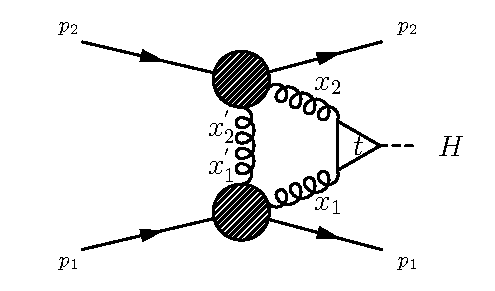
\includegraphics[width=0.8\linewidth]{figures/exclH.pdf}
\caption{Leading order Feynman diagram for the exclusive Higgs production} 
\label{fig:exclHb}
\end{figure}

\par There are several background process that mimic the exclusive Higgs boson signature in the 
ATLAS detector. Justification as to why they qualify to be backgrounds is discussed in Section~\ref{sec:bkgExclH}. 
While estimation of their contribution was in some cases data-driven, Monte Carlo generators were 
used to generate several of them. They are categorized into exclusive and inclusive categories.   

\par The most important exclusive processes that were considered here were the exclusive production 
of \Wpm\ pairs. While exclusive \Wpm\ pairs can be produced through gluon fusion, production through 
photon exchange has a much higher cross section. 500 000 events were generated using \HERWIGPP~\cite{Hpp} 
version 2.6.3, which also handled fragmentation, parton showering and hadronization. This generator 
used the equivalent photon approximation (EPA) introduced in 
Section~\ref{sec:diffPhy}. This generator only handles elastic production (See Figure~\ref{fig:exclWW}). 
This means that estimation of single and double dissociative contributions had to be 
data-driven. 

\par The second most important exclusive processes were the exclusive production of leptons, 
referred to here as the di-leptons. They are produced through photon exchange, so 
the EPA mechanism is used in calculating their 
cross sections. 300 000 elastic \yytautau, 800 000 \yymumu, and 800 \yyee\ events were generated using 
\HERWIGPP.  Just like in the exclusive \Wpm\ pair case, fragmentation, parton showering and hadronization 
were processed within \HERWIGPP\ as well. The single and double dissociative di-lepton samples were 
produced using \LPAIR~\cite{Vermaseren} version 4.0, save for the $\tau\tau$ decay mode. 
\LPAIR\ is a generator dedicated to lepton pair production. Unfortunately, it does not incorporate 
$\tau$ leptons in the generation. Single dissociative \yytautau\ processes were 
therefore generated using \PYTHIA8~\cite{Pythia8}. No Monte Carlo generator 
to date has produced double dissociative \yytautau, so these samples were unavailable.
     
\par Inclusive $WW$ backgrounds have several production modes. These are 
\begin{enumerate}
\item quark-induced $\qqbar\to WW$;
\item gluon-induced $gg\to WW$;
\item and $gg\to H\to WW$, with $m_{\text{H}}=125~\GeV$. 
\end{enumerate} 
The $\qqbar\to WW$ and $gg\to H\to WW$ samples were generated using Powheg 
version 1.0~\cite{Powheg1}. This generator was interfaced to \PYTHIA8\ for parton showering, 
hadronization and simulation of the underlying event. $gg\to WW$ events were generated by 
the \ggww~\cite{gg2WW} generator, interfaced to HERWIG version 6.5 for parton showering, hadronization 
and underlying event generation. In all these generators, the CT10NLO PDF set was used. 
Parton showering, hadronization and underlying event models in \PYTHIA8\ and HERWIG were 
tuned using the AU2~\cite{ATLAS:Pythia8Tune} and the AUET2~\cite{ATLAS:2011Tune} tunes.  
 
\par $W$+jets and $Z$+jets processes were modelled using Alpgen~\cite{Alpgen} interfaced to 
 {Pythia}6~\cite{Pythia6} using the Perugia 2011C~\cite{PerugiaTune} 
tune and CTEQ6L1 PDF~\cite{CTEQ6L1} set. Additional $Z$+jets samples were 
generated with Alpgen interfaced to Herwig+Jimmy. Other $Z$+jets samples, generated using {Powheg+Pythia8} 
and {Sherpa1.4} with CT10 NLO PDF, were also used for additional background studies.  

\par Diboson processes such as $WZ(\gamma^*)$, $W/Z+\gamma$ and $ZZ$ are referred to 
here as $VV$. The $WZ$ and $ZZ$ samples were generated using {Powheg+Pythia} with 
the AU2 tune and CT10 NLO PDF set. $W\gamma$ and $W\gamma^*$ samples were generated, respectively, 
using {Alpgen} (interfaced to {Herwig+Jimmy}) and {Sherpa}.

\par \ttbar\ and single top processes were generated with Powheg and MC@NLO.   
